\documentclass[10pt,a4paper]{article}
\pdfinfoomitdate=1
\pdftrailerid{}
\pdfsuppressptexinfo=15
\usepackage[T1]{fontenc}
\usepackage{lmodern,microtype,graphicx,xcolor,booktabs,tabularx,array,enumitem,titlesec,fancyhdr,hyperref,tikz}
\usetikzlibrary{arrows.meta,positioning}
\usepackage[top=1.45cm,bottom=1.50cm,left=1.65cm,right=1.65cm]{geometry}
\definecolor{navy}{HTML}{163A53}
\definecolor{blue}{HTML}{2B658C}
\definecolor{slate}{HTML}{526775}
\definecolor{ice}{HTML}{EDF4F8}
\definecolor{mist}{HTML}{F2F4F5}
\hypersetup{colorlinks=true,urlcolor=blue,linkcolor=blue,pdftitle={From State Forecasts to Agent Failure Prediction},pdfauthor={Zhijing Wu},pdfsubject={A bounded frozen-model study for Professor Manling Li}}
\setlength{\parindent}{0pt}\setlength{\parskip}{4pt}
\setlist[itemize]{leftmargin=12pt,itemsep=2pt,topsep=3pt,parsep=0pt}
\titleformat{\section}{\fontsize{12.4}{14.2}\selectfont\bfseries\color{navy}}{}{0pt}{}
\titlespacing*{\section}{0pt}{8pt}{4pt}
\pagestyle{fancy}\fancyhf{}\renewcommand{\headrulewidth}{0pt}
\fancyfoot[L]{\fontsize{8.5}{10}\selectfont\color{slate}Zhijing Wu \quad | \quad Research note \quad | \quad 02 November 2026}
\fancyfoot[R]{\fontsize{8.5}{10}\selectfont\color{slate}\thepage\,/\,3}
\newcommand{\eyebrow}[1]{{\small\bfseries\color{blue}\MakeUppercase{#1}}\par\vspace{4pt}}
\newcommand{\captiontext}[1]{{\fontsize{8.8}{10.6}\selectfont\color{slate}#1\par}}
\newcommand{\callout}[1]{\begingroup\setlength{\fboxsep}{7pt}\colorbox{ice}{\parbox{\dimexpr\linewidth-2\fboxsep}{#1}}\endgroup\par}
\newcommand{\smallbody}{\fontsize{9.5}{11.3}\selectfont}
\begin{document}
\eyebrow{Independent research \quad / \quad Agent reliability}
{\fontsize{20.5}{23}\selectfont\bfseries\color{navy}From State Forecasts to\\Agent Failure Prediction\par}
\vspace{4pt}
{\fontsize{12}{14}\selectfont\color{slate}Testing the Incremental Value of Task-Relevant Evidence\par}
\vspace{10pt}
\begin{minipage}[t]{.48\linewidth}
\textbf{Zhijing Wu}\\
Computer Science Undergraduate\\
Sichuan University, China
\end{minipage}\hfill
\begin{minipage}[t]{.49\linewidth}
\textcolor{slate}{Prepared for Professor Manling Li}\\
Multimodal Learning and Language Lab\\
Northwestern University
\end{minipage}
\vspace{10pt}

\callout{\smallbody\textbf{Abstract.} I investigated whether task-relevant summaries of a model's explicit state forecasts improve prediction of later agent failure beyond replay, task feasibility and likelihood diagnostics. I implemented a frozen public SPA evaluation in native Sokoban, preserving 224 episodes and comparing nine fixed feature views on a family-grouped split. In the final at-risk set (124 episodes; four successes), paired gain intervals crossed zero in both likelihood scopes. Forecasts were available in 25/224 initial packets and exact in 1/224. The study establishes a bounded empirical test and a measurement limitation, rather than a new algorithm or a resolved predictive improvement.}

\section{When does a detectable error matter for a decision?}
An agent may describe a state plausibly yet fail under its remaining action budget. The aim is to warn about consequential errors, rather than flag every detectable discrepancy. State accuracy, response dependence and action consistency test different properties of a reply. Task relevance concerns goal consequences; failure prediction concerns later outcomes; causal faithfulness concerns whether stated reasoning drives behavior.

\textbf{Research question.} Do task-relevant summaries of explicit state forecasts improve prediction of later agent failure beyond replay, task feasibility and likelihood diagnostics?

\vspace{3pt}
\begin{center}\begingroup
\hyphenpenalty=10000\relax
\exhyphenpenalty=10000\relax
% Editable vector diagram. Arrows denote data construction, not internal causality.
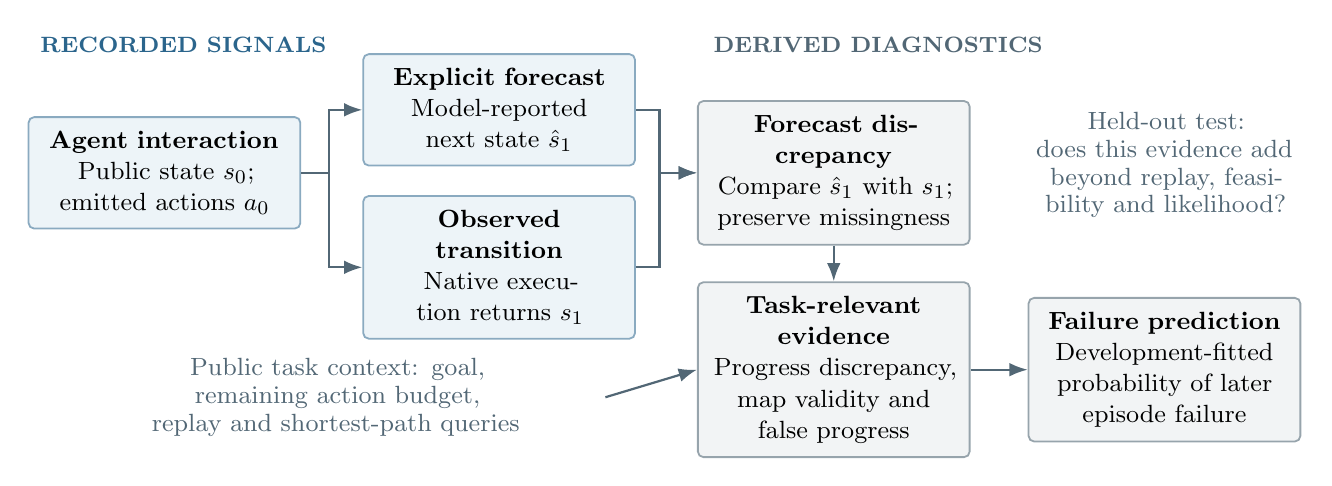
\begin{tikzpicture}[x=1cm,y=1cm,>=Latex,font=\fontsize{9.4}{11.3}\selectfont,
 rec/.style={draw=blue!55,fill=ice,rounded corners=2pt,line width=.65pt,align=center,text width=3.1cm,minimum height=1.02cm,inner sep=5pt},
 der/.style={draw=slate!60,fill=mist,rounded corners=2pt,line width=.65pt,align=center,text width=3.1cm,minimum height=1.02cm,inner sep=5pt},
 flow/.style={->,draw=slate,line width=.8pt},lab/.style={font=\fontsize{8.6}{10}\selectfont,text=slate,align=center}]
\node[font=\footnotesize\bfseries,text=blue,anchor=west] at (.1,4.08) {RECORDED SIGNALS};
\node[font=\footnotesize\bfseries,text=slate,anchor=west] at (8.65,4.08) {DERIVED DIAGNOSTICS};
\node[rec] (agent) at (1.8,2.45) {\textbf{Agent interaction}\\Public state $s_0$; emitted actions $a_0$};
\node[rec] (forecast) at (6.05,3.25) {\textbf{Explicit forecast}\\Model-reported next state $\hat{s}_1$};
\node[rec] (observed) at (6.05,1.25) {\textbf{Observed transition}\\Native execution returns $s_1$};
\node[der] (error) at (10.3,2.45) {\textbf{Forecast discrepancy}\\Compare $\hat{s}_1$ with $s_1$; preserve missingness};
\node[der] (task) at (10.3,-.05) {\textbf{Task-relevant evidence}\\Progress discrepancy, map validity and false progress};
\node[der] (risk) at (14.5,-.05) {\textbf{Failure prediction}\\Development-fitted probability of later episode failure};
\draw[flow] (agent.east) -- ++(.35,0) |- (forecast.west);
\draw[flow] (agent.east) -- ++(.35,0) |- (observed.west);
\draw[flow] (forecast.east) -- ++(.3,0) |- (error.west);
\draw[flow] (observed.east) -- ++(.3,0) |- (error.west);
\draw[flow] (error.south) -- (task.north);
\draw[flow] (task.east) -- (risk.west);
\node[lab,text width=6.6cm,anchor=east] (goal) at (7.4,-.4) {Public task context: goal, remaining action budget,\\replay and shortest-path queries};
\draw[flow] (goal.east) -- (task.west);
\node[lab,text width=3.3cm] at (14.5,2.55) {Held-out test:\\does this evidence add beyond replay, feasibility and likelihood?};
\end{tikzpicture}

\endgroup
\end{center}
\captiontext{\textbf{Figure 1. Research question and evidence construction.} Blue boxes are recorded signals; slate boxes are derived diagnostic features or fitted predictions. A forecast and an observed transition are compared, then interpreted with the same public goal and budget. Arrows describe evidence flow, not a causal claim about internal reasoning. Missing forecasts are never filled from simulator truth.}

\section{What I contributed to this investigation}
\begin{itemize}
\item A controlled frozen-release experiment with saved prompts, raw tokens, native transitions, fixed feature views and strong replay/task comparisons.
\item A paired held-out test that separates a tiny point estimate from a resolved gain, while exposing sparse forecasts, low event counts and an unavailable primary calibration fit.
\item A concrete follow-up question: which forecast errors become informative after task feasibility and ordinary replay are already known?
\end{itemize}

\section{Relation to Professor Li's research}
RAGEN-2 already studies reasoning collapse and cross-input diagnostics [1]; VAGEN and SPA study state/transition reasoning or supervision [2,3]. My question concerns a narrower reliability boundary in multi-turn world-model agents: whether explicit forecast errors carry additional \emph{decision-relevant} evidence. This connects to agentic RL and embodied-agent reliability without treating this symbolic task as an embodied-system reproduction.


\newpage
\eyebrow{Experimental design \quad / \quad Implemented evidence pipeline}
{\fontsize{17}{20}\selectfont\bfseries\color{navy}One controlled pipeline, nine feature views\par}
\vspace{6pt}
\smallbody
\begin{minipage}[t]{.49\linewidth}
\textbf{Execution.} Public SPA Sokoban release (1.543B unique parameters), fixed weights; native one-box $6\times6$ grids. Ten action attempts, five model turns; temperature 0.7, top-$p$ 0.8, top-$k$ 20 and 400 new tokens per response.
\end{minipage}\hfill
\begin{minipage}[t]{.48\linewidth}
\textbf{Prediction landmark.} After the first proposed action batch and returned native observation; zero mapped actions are possible. Failure is no success within the horizon. Exclude cases already complete, terminal or out of budget.
\end{minipage}\par
\vspace{8pt}
\noindent\makebox[\linewidth][c]{\begingroup
\hyphenpenalty=10000\exhyphenpenalty=10000
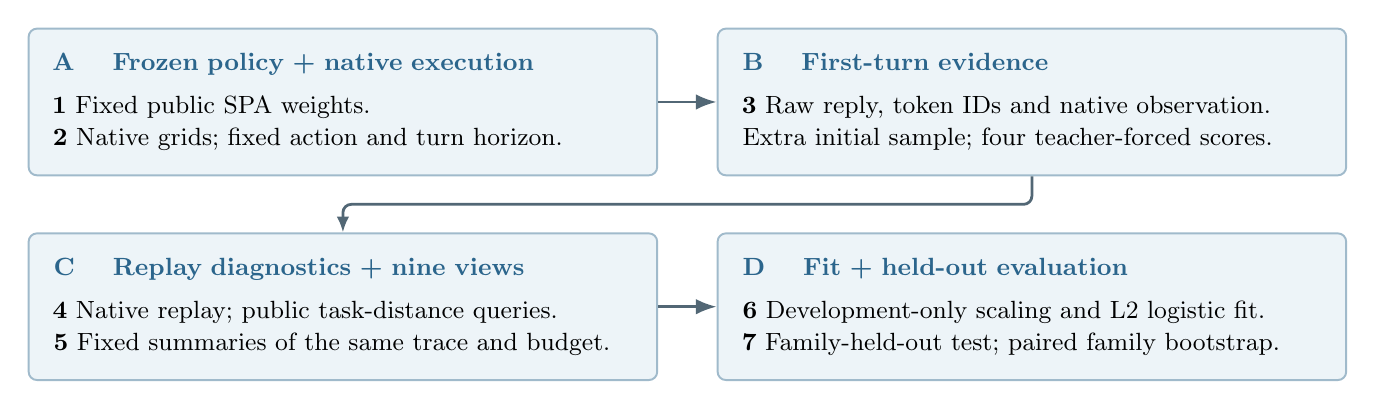
\begin{tikzpicture}[x=1cm,y=1cm,>=Latex,
  font=\fontsize{9.5}{11.5}\selectfont,
  panel/.style={draw=blue!45,fill=ice,rounded corners=3pt,line width=.7pt,
    text width=7.35cm,minimum height=1.72cm,inner sep=9pt,align=left},
  flow/.style={->,draw=slate,line width=1pt,rounded corners=3pt}]
\node[panel] (a) at (0,0) {\textcolor{blue}{\textbf{A \quad Frozen policy + native execution}}\\[4pt]
  \textbf{1} Fixed public SPA weights.\\
  \textbf{2} Native grids; fixed action and turn horizon.};
\node[panel] (b) at (8.75,0) {\textcolor{blue}{\textbf{B \quad First-turn evidence}}\\[4pt]
  \textbf{3} Raw reply, token IDs and native observation.\\
  Extra initial sample; four teacher-forced scores.};
\node[panel] (c) at (0,-2.6) {\textcolor{blue}{\textbf{C \quad Replay diagnostics + nine views}}\\[4pt]
  \textbf{4} Native replay; public task-distance queries.\\
  \textbf{5} Fixed summaries of the same trace and budget.};
\node[panel] (d) at (8.75,-2.6) {\textcolor{blue}{\textbf{D \quad Fit + held-out evaluation}}\\[4pt]
  \textbf{6} Development-only scaling and L2 logistic fit.\\
  \textbf{7} Family-held-out test; paired family bootstrap.};
\draw[flow] (a.east)--(b.west);
\draw[flow,-{Latex[length=2mm,width=1.6mm]}] (b.south)--(8.75,-1.3)--(0,-1.3)--(c.north);
\draw[flow] (c.east)--(d.west);
\end{tikzpicture}
\endgroup
}\par\vspace{3pt}
\captiontext{\textbf{Figure 2. Implemented architecture.} Four stages preserve all seven operations. Every view is charged the same recorded evidence packet; this compares summaries at equal spend, not optimal online allocation. All stages were executed.}

\section{A split designed around task families}
\begin{tabularx}{\linewidth}{@{}Xrrr@{}}
\toprule
& Development & Calibration & Final\\\midrule
Fixed boards & 64 & 32 & 128\\
D4 wall-plus-target families & 50 & 27 & 106\\
At-risk episodes & 63 & 30 & 124\\
At-risk successes / failures & 2 / 61 & 0 / 30 & 4 / 120\\\bottomrule
\end{tabularx}
\vspace{2pt}
No family crosses splits. Standardization and L2 logistic regression ($C=1$) use development labels only; no final-set tuning. Family separation does not prove unseen-wall or pretraining-disjoint generalization.

\section{Nine fixed feature views}
{\setlength{\tabcolsep}{4pt}\renewcommand{\arraystretch}{1.06}
\begin{tabularx}{\linewidth}{@{}p{4.5cm}rX@{}}
\toprule
View & Columns & Evidence used / comparison role\\\midrule
Development prior & 0 & Smoothed development failure rate.\\
State + format & 11 & Current-state scores and missingness.\\
Ordinary replay & 12 & Forecast/native agreement; no-op indicator.\\
Likelihood proxy & 9 & Own NLL; finite cross-input dependence.\\
State + replay + likelihood & 18 & Combined generic diagnostics.\\
Two-sample disagreement & 23 & Extra initial-sample disagreement.\\
Replay + task / deadlock & 25 & Goal distance, progress and feasibility.\\
Task-relevance candidate & 34 & Nine added forecast/task summaries.\\
Matched generic interactions & 34 & Nine generic terms as a capacity control.\\\bottomrule
\end{tabularx}}
\vspace{2pt}
Nonprior views include format, action, budget and output-length controls. They reuse the same episodes, not nine independent experiments. Equal columns do not guarantee equal effective capacity.

\section{Availability and likelihood are separate measurements}
\begin{minipage}[t]{.42\linewidth}\vspace{0pt}
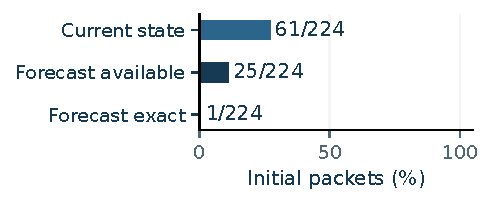
\includegraphics[width=\linewidth]{figures/availability.pdf}
\captiontext{All 224 initial packets. All 25 forecasts are explicit grids; one is exact. Current-state evidence also permits explicit entity coordinates.}
\end{minipage}\hfill
\begin{minipage}[t]{.55\linewidth}\vspace{0pt}
\textbf{Registered:} actual generated token IDs through the first closing think tag; this may measure formatting.

\textbf{Full tail:} entire actual first-response tail; same own/three-reference scheme. 896 teacher-forcing passes, zero extra sampling. Planned after collection began, before analysis; added scoring cost is charged.

Finite length-normalized proxies, not exact MI or full RAGEN-2 reproductions. Dependence and correctness do not establish causal faithfulness [4].
\end{minipage}

\newpage
\eyebrow{Results \quad / \quad Interpretation and proposed next steps}
{\fontsize{17}{20}\selectfont\bfseries\color{navy}No resolved increment over the strong baseline\par}
\vspace{5pt}
\callout{\smallbody\textbf{Read with the low-event warning.} The final at-risk set has \textbf{124 episodes: four successes and 120 failures across 102 layout families}. The primary calibration map cannot be fitted: all 30 at-risk calibration episodes failed. The primary probabilities remain uncalibrated.}
\vspace{4pt}
\noindent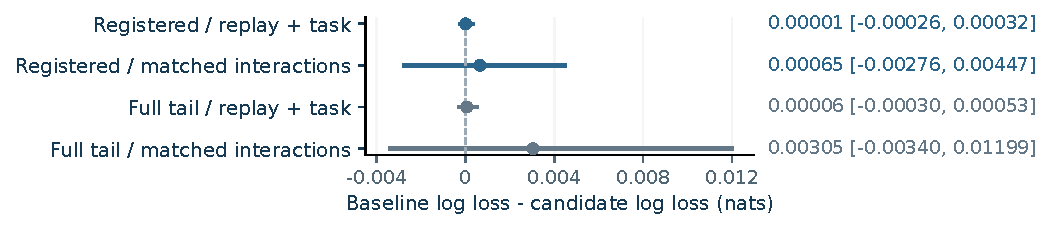
\includegraphics[width=\linewidth]{figures/paired_gain.pdf}\par\vspace{2pt}
\captiontext{\textbf{Figure 3. Paired held-out log-loss gain.} Positive values favor the task-relevance candidate. Bars are 95\% percentile intervals from 2,000 paired wall-plus-target-family resamples, conditional on the development fit. They exclude full retraining uncertainty; comparisons are exploratory. Both replay/task intervals and both matched-interaction intervals cross zero.}

\vspace{4pt}
{\fontsize{9.1}{10.7}\selectfont\setlength{\tabcolsep}{4pt}\renewcommand{\arraystretch}{1.03}
\begin{tabularx}{\linewidth}{@{}Xrrrr@{}}
\toprule
& \multicolumn{2}{c}{Held-out log loss $\downarrow$} & \multicolumn{2}{c}{Brier score $\downarrow$}\\
View & Registered & Full tail & Registered & Full tail\\\midrule
Development prior & 0.1449 & 0.1449 & 0.0314 & 0.0314 \\
State + format & 0.1064 & 0.1064 & 0.0289 & 0.0289 \\
Ordinary replay & 0.0947 & 0.0947 & 0.0272 & 0.0272 \\
Likelihood proxy & 0.1152 & 0.1028 & 0.0296 & 0.0283 \\
State + replay + likelihood & 0.1054 & 0.0920 & 0.0282 & 0.0266 \\
Two-sample disagreement & 0.1040 & 0.0901 & 0.0282 & 0.0268 \\
Replay + task / deadlock & 0.0395 & 0.0429 & 0.0097 & 0.0113 \\
Task-relevance candidate & 0.0395 & 0.0429 & 0.0096 & 0.0112 \\
Matched generic interactions & 0.0402 & 0.0459 & 0.0103 & 0.0131 \\
\bottomrule
\end{tabularx}}

\section{What this finding means}
The replay/task baseline already captures much of the predictive signal in this cohort. The candidate's additional summaries vary, but their tiny point gains do not resolve an increment. Sparse forecasts (25/224) and rare exact forecasts (1/224) limit the opportunity to measure task-relevant forecast error. This is an inconclusive incremental comparison, not a failed execution, proof of equivalence or evidence that better forecasts cannot help. Novelty remains unestablished (B).

\textbf{Limits.} One small frozen model and deterministic, fully observed Sokoban restrict generalization. Only four final at-risk successes trigger the preset low-event warning. All-episode calibration sensitivity has two successes in 32 calibration cases and does not replace the unavailable primary fit. The inference interface was adapted during qualification; historical generator identity and the RAGEN leaf commit remain unverified. No causal intervention on internal reasoning was performed.

\vspace{5pt}
\noindent\begingroup
\hyphenpenalty=10000\relax
\exhyphenpenalty=10000\relax
% All stages below are proposed future research; none is claimed completed.
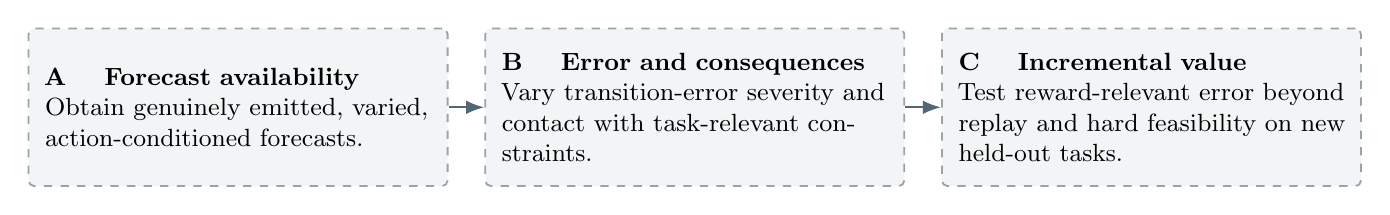
\begin{tikzpicture}[x=1cm,y=1cm,>=Latex,font=\fontsize{9.1}{11}\selectfont,
 future/.style={draw=slate!60,fill=mist,dashed,rounded corners=2pt,text width=4.9cm,align=left,minimum height=2.00cm,inner sep=6pt,line width=.65pt}]
\node[future] (a) at (0,0) {\textbf{A \quad Forecast availability}\\Obtain genuinely emitted, varied, action-conditioned forecasts.};
\node[future] (b) at (5.8,0) {\textbf{B \quad Error and consequences}\\Vary transition-error severity and contact with task-relevant constraints.};
\node[future] (c) at (11.6,0) {\textbf{C \quad Incremental value}\\Test reward-relevant error beyond replay and hard feasibility on new held-out tasks.};
\draw[->,draw=slate,line width=.8pt] (a.east)--(b.west);
\draw[->,draw=slate,line width=.8pt] (b.east)--(c.west);
\end{tikzpicture}

\endgroup
\par\vspace{2pt}
\captiontext{\textbf{Figure 4. Proposed future research, not completed experiments.} First qualify forecast availability and event counts; then test task consequence on a new held-out population with replay/feasibility and matched-information controls. None of these stages has been launched.}
\vspace{4pt}
\textbf{Discussion question.} Under what conditions does an agent's forecast error become decision-relevant, rather than merely detectable?

\vspace{5pt}
{\fontsize{8.4}{10.0}\selectfont\color{slate}
\textbf{References.} [1] Z. Wang et al. \emph{RAGEN-2: Reasoning Collapse in Agentic RL}. ICML 2026, PMLR 306.
[2] K. Wang et al. \emph{VAGEN}. NeurIPS 2025.
[3] S. Chen et al. \emph{Why Do LLM Agents Fail in Exploring New Environments? A World-Modeling Perspective}. arXiv:2510.15047v2.
[4] T. Lanham et al. \emph{Measuring Faithfulness in Chain-of-Thought Reasoning}. arXiv:2307.13702v1.

\textbf{Reproducibility.} Editable diagrams, plot code, references, sanitized claim checks and file hashes accompany this note. Token/prompt, native/public replay and independent statistical checks passed. Original 128 records are byte-identical; the resumed 96 retain batches 16--27. No new experiment was run for this document. Public aggregates reproduce figures and tables; raw trajectories and weights are excluded. \href{https://github.com/ZhijingWu/agent-forecast-failure-prediction}{\textbf{Code and public evidence: github.com/ZhijingWu/agent-forecast-failure-prediction}}.}
\end{document}
